\documentclass[a4paper,12pt]{article}

\usepackage{cmap}
\usepackage[T2A]{fontenc}
\usepackage[utf8x]{inputenc}
\usepackage[english, russian]{babel}

\usepackage{misccorr} % в заголовках появляется точка, но при ссылке на них ее нет
\usepackage{amssymb,amsfonts,amsmath,amsthm}  
\usepackage{indentfirst}
\usepackage[usenames,dvipsnames]{color} 
\usepackage[unicode,hidelinks]{hyperref}
% \hypersetup{%
%     pdfborder = {0 0 0}
% }
\usepackage{makecell,multirow} 
\usepackage{ulem}
\usepackage{graphicx,wrapfig}
\graphicspath{{img/}}
\usepackage{geometry}
\geometry{left=2cm,right=2cm,top=3cm,bottom=3cm,bindingoffset=0cm,headheight=15pt}
\usepackage{fancyhdr} 
\linespread{1.2} 
\frenchspacing 
\renewcommand{\labelenumii}{\theenumii)} 
% \usepackage{caption}
%%%%%%%%%%%%%%%%%%%%%%%%%%%%%%%%%%%%%%%%%%%%%%%%%%%%%%%%%%%%%%%%%%%%%%%%%%%%%%%
%%%%%%%%%%%%%%%%%%%%%%%%%%%%%%%%%%%%%%%%%%%%%%%%%%%%%%%%%%%%%%%%%%%%%%%%%%%%%%%

\def\labauthor{Сарафанов Ф.Г., Платонова М.В.}
\def\labauthors{\labauthor}
\def\labnumber{3}
\def\labtheme{Исследование матриц рассеяния \\[0.4em] волноводных узлов}

%%%%%%%%%%%%%%%%%%%%%%%%%%%%%%%%%%%%%%%%%%%%%%%%%%%%%%%%%%%%%%%%%%%%%%%%%%%%%%%
	%применим колонтитул к стилю страницы
\pagestyle{fancy} 
	%очистим "шапку" страницы
\fancyhead{} 
	%слева сверху на четных и справа на нечетных
\fancyhead[L]{\labauthors} 
	%справа сверху на четных и слева на нечетных
\fancyhead[R]{Отчёт по лабораторной работе №\labnumber} 
	%очистим "подвал" страницы
\fancyfoot{} 
	% номер страницы в нижнем колинтуле в центре
\fancyfoot[C]{\thepage} 

%%%%%%%%%%%%%%%%%%%%%%%%%%%%%%%%%%%%%%%%%%%%%%%%%%%%%%%%%%%%%%%%%%%%%%%%%%%%%%%

\usepackage{float}
\usepackage[mode=buildnew]{standalone}
\usepackage{tikz} 
% \usepackage{subcaption}
\usepackage{tikz,csvsimple}
\usetikzlibrary{scopes}
\usetikzlibrary{%
     decorations.pathreplacing,%
     decorations.pathmorphing,%
    patterns,%
    calc,%
    scopes,%
    arrows,%
    % arrows.spaced,%
}
\makeatletter
\newif\if@gather@prefix 
\preto\place@tag@gather{% 
  \if@gather@prefix\iftagsleft@ 
    \kern-\gdisplaywidth@ 
    \rlap{\gather@prefix}% 
    \kern\gdisplaywidth@ 
  \fi\fi 
} 
\appto\place@tag@gather{% 
  \if@gather@prefix\iftagsleft@\else 
    \kern-\displaywidth 
    \rlap{\gather@prefix}% 
    \kern\displaywidth 
  \fi\fi 
  \global\@gather@prefixfalse 
} 
\preto\place@tag{% 
  \if@gather@prefix\iftagsleft@ 
    \kern-\gdisplaywidth@ 
    \rlap{\gather@prefix}% 
    \kern\displaywidth@ 
  \fi\fi 
} 
\appto\place@tag{% 
  \if@gather@prefix\iftagsleft@\else 
    \kern-\displaywidth 
    \rlap{\gather@prefix}% 
    \kern\displaywidth 
  \fi\fi 
  \global\@gather@prefixfalse 
} 
\newcommand*{\beforetext}[1]{% 
  \ifmeasuring@\else
  \gdef\gather@prefix{#1}% 
  \global\@gather@prefixtrue 
  \fi
} 
\makeatother

\usepackage{booktabs}
\usepackage{pgfplots, pgfplotstable}

\usepackage[outline]{contour}
\usepackage{tocloft}
\renewcommand{\cftsecleader}{\cftdotfill{\cftdotsep}} % for parts
% \renewcommand{\cftchapleader}{\cftdotfill{\cftdotsep}} % for chapters
\usepackage{pgfplots,pgfplotstable,booktabs,colortbl}

% \renewcommand{\arraystretch}{1.5} 

\pgfkeys{/pgf/number format/.cd,
		fixed,  1000 sep={\,}}

\pgfplotstableset{
	% multicolumn names, % allows to have multicolumn names
	% header=has colnames,
	% dec sep align,
	col sep=tab, % the seperator in our .csv file
	% fixed zerofill, 
	% precision=4,
	columns/1/.style={
		column name={1},
		string type,
	},	
	columns/2/.style={
		column name={2},
		string type,
	},	
	columns/3/.style={
		column name={3},
		string type,
	},	
	columns/Skm/.style={
		column name={$S_{km}$},
		string type,
	},	
	columns/S/.style={
		column name={$S_{km}$},
		string type,
		column type = {l},
	},	
	columns/N/.style={
		column name={№},
		precision=0,
		% fixed zerofill, 	
		% % column type/.add={|}{},
	},
	columns/Imax/.style={
		column name={$I_{\max}$},
		dec sep align,
		precision=0,
	},
	columns/Imin/.style={
		column name={$I_{\min}$},
		dec sep align,
		precision=1,
	},
	columns/Gamma/.style={
		column name={$|\Gamma|$},
		dec sep align,
		precision=2,
	},
	columns/phi/.style={
		column name={$\varphi_H$},
		dec sep align,
		precision=2,
	},
	columns/zmin/.style={
		column name={$z_{\min}$, см},
		dec sep align,
		precision=2,
	},
	empty cells with={\textbf{--}},
	every head row/.style={
	before row={\toprule},
	after row={
		\midrule}
		},
	every last row/.style={after row=\bottomrule},
	every row/.style={after row=\midrule}, 
	create on use/Gamma/.style={
	    create col/expr={
	    	(sqrt(\thisrow{Imax}/\thisrow{Imin})-1)/(sqrt(\thisrow{Imax}/\thisrow{Imin})+1)%*\thisrow{ul5}/\thisrow{u}
	    }
	},
	create on use/phi/.style={
	    create col/expr={
	    	4*pi*abs(\thisrow{zmin}-5.145)/5.47-pi
	    }
	},
	columns={N,Skm,1,2,3,Imax,Imin,zmin,Gamma,phi,S},		
	% dec zerofill
	% fixed,fixed zerofill,
	% precision=3
	% every even column/.style={%
	% 	% column type/.add={>{\columncolor[gray]{.8}}}{}
	% },
	% every even row/.style={%
	% 	before row={\rowcolor[gray]{0.95}},
	% },	
	% every head row/.style={
 %        before row={
 %        	& & \multicolumn{3}{c}{Номер входа} & \\ \toprule
 %        },
 %        after row=\midrule
	% },
	}%

\pgfplotsset{compat=newest}
\usepackage{physics}
\usepackage{mathtools}
\mathtoolsset{showonlyrefs=true}
\newcommand\Smat{\hat { \mathbf { S } }}


\begin{document}

\begin{titlepage}
\begin{center}

{\textsc{Нижегородский государственный университет имени Н.\,И. Лобачевского}}
\vskip 2pt \hrule \vskip 3pt
{\textsc{Радиофизический факультет}}

\vfill


{{\LARGE Отчет по лабораторной работе №\labnumber}\vskip 12pt {\Huge \bfseries \labtheme}}

	
\vspace{2cm}
{\large Работу выполнили студенты \\[-0.25em] 430 группы радиофизического факультата \\[0.5em] {\Large \bfseries \labauthor}}

% \vspace{0.5cm}
% {e-mail: sfg180@yandex.ru}

% \vspace{2cm}

\end{center}

\vfill
	
% \begin{flushright}
% 	{Выполнили студенты 430 группы\\ \labauthor}%\vskip 12pt Принял:\\ Менсов С.\,Н.}
% \end{flushright}
	
% \vfill
	
\begin{center}
	{Нижний Новгород, \today}
\end{center}

\end{titlepage}

\tableofcontents
\newpage

\section*{Введение}
\addcontentsline{toc}{section}{Введение}
\label{sec:input}

В данной работе изучаются с помощью матричного анализа волноводные узлы -- шестиполюсники. У них с помощью измерительной линии измеряются величины, позволяющие рассчитать коэффициенты матрицы рассеяния шестиполюсников $S_{km}$. 

На основе рассчитанной матрицы рассеяния $S$ конкретного шестиполюсников можно попытаться решить обратную задачу: сделать на основе полученных данных предположение о возможных конструктивных вариантах волноводных узлов, находящихся внутри шестиполюсников.

\section{Теоретические сведения}
\subsection{Матрица рассеяния шестиполюсника}

Рассмотрим трехплечий волноводный узел (шестиполюсник), изображенный на рис. 1. В каждом плече выберем \textbf{плоскость отсчета} (сечение), в котором будем находить отношения амплитуд полей отраженной и падающей волн.

\begin{figure}[h!]
	\centering
	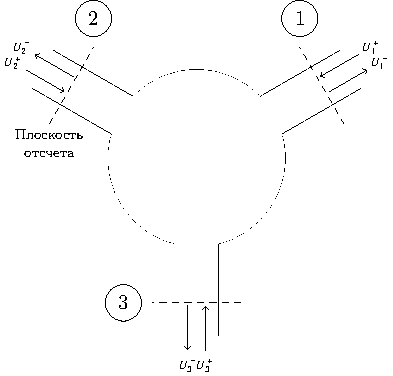
\includegraphics[scale=1.5]{ris/ris1}
	\caption{Схема трехплечего узла (шестиполюсника)}
	\label{fig:figure1}
\end{figure}

Обозначим комплексные амплитуды полей входящих (падающих) в узел волн через $U_m^+$, а амплитуды выходящих (отраженных) волн через $U_k^-$. 
Величины $U_k^-$ зависят от амплитуд и фаз полей волн, входящих во все плечи узла, причем эти зависимости являются линейными в силу линейности уравнений Максвелла (предполагается, что нелинейных элементов в узле нет). 
Связь между амплитудами полей в плечах узла записывается в виде:
\begin{gather}
	\label{eq:usu}
	{ U _ { 1 } ^ { - } = S _ { 11 } U _ { 1 } ^ { + } + S _ { 12 } U _ { 2 } ^ { + } + S _ { 13 } U _ { 3 } ^ { + } } \\ 
	{ U _ { 2 } ^ { - } = S _ { 21 } U _ { 1 } ^ { + } + S _ { 22 } U _ { 2 } ^ { + } + S _ { 23 } U _ { 3 } ^ { + } } \\
	{ U _ { 3 } ^ { - } = S _ { 31 } U _ { 1 } ^ { + } + S _ { 32 } U _ { 2 } ^ { + } + S _ { 33 } U _ { 3 } ^ { + } } 
\end{gather}
где $S_{km}$ ---  комплексные коэффициенты, характеризующие волноводный узел. 

Систему уравнений \eqref{eq:usu} удобно записать в матричной форме
\begin{equation}
	\left( \begin{array} { c } { U _ { 1 } ^ { - } } \\ { U _ { 2 } ^ { - } } \\ { U _ { 3 } ^ { - } } \end{array} \right) = \Smat \left( \begin{array} { l } { U _ { 1 } ^ { + } } \\ { U _ { 2 } ^ { + } } \\ { U _ { 3 } ^ { + } } \end{array} \right), \quad\text{где}\quad
	\Smat = \left( \begin{array} { c c c } { S _ { 11 } } & { S _ { 12 } } & { S _ { 13 } } \\ { S _ { 21 } } & { S _ { 22 } } & { S _ { 23 } } \\ { S _ { 31 } } & { S _ { 32 } } & { S _ { 33 } } \end{array} \right)
\end{equation}

Матрица $\Smat$ называется матрицей рассеяния, или $S$-матрицей (от англ. scattering -- рассеяние).

Из определения элементов матрицы рассеяния следует, что для пассивных узлов, не обладающих свойством усиления мощности, модули коэффициентов передачи и отражения не могут превышать единицы.
\subsection{Свойства матрицы рассеяния}


\paragraph{Взаимный узел.} Волноводные узлы, в которых отсутствуют элементы с гиротропными свойствами (например, намагниченный феррит), являются взаимными устройствами. Их матрицы рассеяния симметричны относительно главной диагонали

\begin{equation}
	S_{mk}=S_{km}
\end{equation}

Верно и обратное утверждение: если волноводное устройство описывается симметричной матрицей рассеяния, то оно является взаимным.

Отметим, что для взаимных узлов свойства матриц, доказанные для строк, выполняются и для столбцов, и наоборот.

\paragraph{Волноводное устройство без потерь.} Матрица рассеяния волноводного устройства без потерь является унитарной, т.е.
\begin{equation}
	\Smat^T\Smat^*= \hat { \mathbf { I } }
\end{equation}
Можно показать \cite{met}, что для унитарной матрицы выполняются следующие свойства:
\begin{equation}
	\sum _ { m = 1 } ^ { N } S _ { m k } S _ { m k } ^ { * } = \sum _ { m = 1 } ^ { N } \left| S _ { m k } \right| ^ { 2 } = 1
\end{equation}
т.е. сумма квадратов модулей всех матричных элементов любого столбца матрицы рассеяния узла без потерь равна единице.

Второе свойство --- для любой пары столбцов сумма (по строкам) произведений каждого матричного элемента из одного столбца на комплексно сопряженный элемент из той же строки другого столбца равна нулю:
\begin{equation}
	\sum _ { m = 1 } ^ { N } S _ { m l } S _ { m k } ^ { * } = 0 , \quad k \neq l
\end{equation}

\paragraph{Смещение плоскости отсчета.} Предположим, что известна матрица рассеяния при некотором положении плоскости отсчета $z = 0$ в $m$-ом плече узла. При смещении этого сечения на расстояние $l_m$ в направлении распространения падающей волны (по направлению к узлу) новая матрица рассеяния может быть построена по следующим формулам:
\begin{equation}
	\begin{array} { l } { S _ { m k } ^ { \prime } = S _ { m k } e ^ { i \left( h _ { m } l _ { m } + h _ { k } l _ { k } \right) } } \\ { S _ { m m } ^ { \prime } = S _ { m m } e ^ { i 2 h _ { m } l _ { m } } } \end{array}
\end{equation}
где $h_m$ -- постоянная распространения волны в $m$-ом плече. 

Таким образом, изменение плоскости отсчета приводит лишь к изменению фазы коэффициентов матрицы рассеяния, не меняя их абсолютного значения. 


\newpage
\section{Эксперимент}
\subsection{Используемое оборудование}

\begin{enumerate}
	\item СВЧ-генератор Г4-225, в режиме работы на частоте 8.5 ГГц с установленным значением затухания $-4$ дБ
	\item Три шестиполюсника, пластина для закорачивания волновода и две согласованные нагрузки
	\item Измерительная волноводная линия 33-И с кристаллическим детектором, в цепи которого включен амперметр
\end{enumerate}

\subsubsection{Определение коэффициента отражения от нагрузки c помощью измерительной линии}

Измерение элементов матрицы $\Smat$ производится с помощью измерительной линии передачи. Линия передачи позволяет измерить фазу и модуль коэффициента отражения $\Gamma$:

\begin{equation}
	\Gamma=\left(\frac{U_\text{пад}}{U_\text{отр}}\right)_H= | \Gamma | e ^ { i \varphi _ { \mathrm { H } } }
\end{equation}

Модуль коэффициента отражения определялся через коэффициент стоячей волны $K$:
\begin{equation}
	| \Gamma | = \frac { K - 1 } { K + 1 }
\end{equation}

Измерение $K$ производилось путем перемещения вдоль измерительной линии (ИЛ) зонда, показания которого связаны с высокочастотным напряжением в данном сечении линии. 

Для детектирования СВЧ сигнала зонда в ИЛ стоит кристаллический детектор. 
При этом зависимость между током детектора $I$ и приложенным высокочастотным напряжением $|U|$ является нелинейной, и при малых значениях переменного напряжения детектор имеет характеристику $I=f(|U|)$, близкую к квадратичной. В этом случае ток детектора
\begin{equation}
	I=\alpha|U|^2,
\end{equation}
где $\alpha$ --- параметр, зависящий от свойств детектора.

В максимуме и в минимуме распределения поля в линии имеем
\begin{equation}
	I _ { \max } = \alpha | U | _ { \min x } ^ { 2 } , \quad I _ { \min } = \alpha | U | _ { \min } ^ { 2 }
\end{equation}
откуда
\begin{equation}
	\mathrm { K } = \sqrt { \frac { I _ { \mathrm { max } } } { I _ { \mathrm { min } } } }
\end{equation}

Величина фазы коэффициента отражения в сечении $z$ ($z<0$) --- $\psi=\phi_H+2hz$ определялась следующим образом: определялось положение минимума напряжения в ИЛ
% \footnote{При характеристике детектора, близкой к квадратичной, минимум тока детектора никогда не бывает четко выраженным, особенно при небольших К. Для повышения точности отсчета положений минимумов $z_{\min}$ применяют метод <<вилки>>, состоящий в определении двух положений зонда $z_1$ и $z_2$ при одинаковых показаниях индикатора и вычислении $z_{\min}$ по формуле $z_{\min}=(z_1+z_2)/2$.}
 относительно плоскости присоединения нагрузки. Для этого был сначала определен т.н. \textbf{условный конец линии} -- сечение волновода, соответствующее минимуму напряжения при коротком замыкании линии ($z^0_{min}$).
Обозначив расстояние от условного конца линии $z^0_{min}$ до ближайшего минимума напряжения $z_{min}$ \textbf{со стороны генератора} при включенной нагрузке через 
\begin{equation}
	\Delta z _ { \min } \equiv z _ { \min } ^ { 0 } - z _ { \min } = \left| z _ { \min } - z _ { \min } ^ { 0 } \right| =- \left( z _ { \min } - z _ { \min } ^ { 0 } \right)
\end{equation}

И тогда фаза коэффициента отражения (с учетом выражения $h=2\pi/\lambda_B$) определяется формулой
\begin{equation}
	\varphi _ { \mathrm { H } } = 4 \pi \frac { \Delta z _ { \mathrm { min } } } { \lambda _ { \mathrm { B } } } - \pi
\end{equation}

\subsection{Фиксация условного конца линии. Длина волны в волноводе}

Закоротив с помощью короткозамыкателя измерительную линию, зонд измерительной линии установили в ближайший к концу линии узел стоячей волны. 

При этом координата этого узла взята за условный конец линии: 
\begin{equation}
 	z^0_{min}=5.145\text{ см}
 \end{equation}
Измерить длину волны в волноводе $\lambda_B$.

Продвигая зонд в сторону генератора до ближайшего узла, нашли значение длины волны в волноводе:
\begin{equation}
	\frac{\lambda_B}{2}=5.145-2.41=2.735\text{ см}
	\quad\Rightarrow\quad \lambda_B=5.47\text{ см}
\end{equation}

При этом расчетная длина волны $5.49$ см, что неплохо согласуется с экспериментом.

\subsection{Проверка согласованных нагрузок}

Присоединив к скрутке волновода на конце измерительной линии каждую из двух используемых при выполнении работы согласованных нагрузок, определили для них коэффициенты отражения $\Gamma_{H1,2}$. Для точного расчета по приведенным в теории формулам нужно, чтобы они были равны нулю, соответственно для приближенного расчета достаточно близости к нулю. 

Измеренные значения $\Gamma_{H1}=0.0825,\Gamma_{H2}=0.095$, достаточно малы для применения расчетных формул.

\subsection{Измерение параметров шестиполюсников и расчет $S_{km}$}

Для каждого из трех шестиполюсников было осуществлено 6 экспериментов, для измерения диагональных и недиагональных элементов.

\subsubsection{Процедура измерения диагональных элементов}
Пронумеровав условно плечи шестиполюсника как 1,2,3 и зафиксировав их расположение, 
к плечу 1 подключили генератор (Г), а плечи 2 и 3 нагрузили согласованными нагрузками (Н). 

При этом матричное уравнение упрощается, и можно показать, что

\begin{equation}
	\Gamma _ { 11 } = S _ { 11 } = \left| \Gamma _ { 11 } \right| e ^ { i \varphi _ { 11 } }
\end{equation}

Присоединяя генератор поочередно к плечам 2 и 3, определили элементы $S_{22}$ и $S_{33}$.

\subsubsection{Процедура измерения недиагональных элементов}

Для измерения недиагональных элементов, 2 плечо замыкается накоротко, 3 плечо подключается к согласованной нагрузке, и тогда
\begin{equation}
	\Gamma _ { 12 } = S _ { 11 } - \frac { S _ { 12 } S _ { 21 } } { 1 + S _ { 22 } }
\end{equation}
Тогда для произведения недиагональных элементов матрицы рассеяния имеем
\begin{equation}
	S _ { 12 } S _ { 21 } = \left( 1 + S _ { 22 } \right) \left( S _ { 11 } - \Gamma _ { 12 } \right),\qquad\text{1--генератор 2--замыкание 3--нагрузка}
\end{equation}
Поскольку диагональные элементы $S_{mm}$ известны (из предыдущих экспериментов), а коэффициент отражения $\Gamma_{12}=|\Gamma_{12}|e^{i\phi_{12}}$ можно найти с помощью измерительной линии, то этот эксперимент дает возможность определить произведение $S_{12}S_{21}$.
При такой методике измерения невозможно определить отдельно элементы $S_{12}$ и $S_{21}$, однако, если шестиполюсник не содержит невзаимных элементов, то $S_{12} = S_{21}$, и тогда

Расчетные формулы:
\begin{equation}
	S _ { 12 }^2 = \left( 1 + S _ { 22 } \right) \left( S _ { 11 } - \Gamma _ { 12 } \right),\qquad\text{1--генератор 2--замыкание 3--нагрузка}
\end{equation}
\begin{equation}
	S _ { 13 } ^ { 2 } = \left( 1 + S _ { 33 } \right) \left( S _ { 11 } - \Gamma _ { 13 } \right),\qquad\text{1--генератор 2--нагрузка 3--замыкание}
\end{equation}
\begin{equation}
	S _ { 23 } ^ { 2 } = \left( 1 + S _ { 33 } \right) \left( S _ { 22 } - \Gamma _ { 23 } \right),\qquad\text{1--нагрузка 2--генератор 3--замыкание}
\end{equation}

Для расчета корней из комплексных чисел для оптимизации временных затрат использовалась система \textbf{Wolfram Mathematica}.

\newpage
\subsubsection{Результаты измерений и расчётов}

\begin{table}[h!]
	\caption{Измерения характеристик шестиполюсника №1}
	\label{tab:6s1}
	\vspace{1em}
	\centering
	\pgfplotstabletypeset[]{data/tab1.tsv}
\end{table}






\begin{table}[h!]
	\caption{Измерения характеристик шестиполюсника №2}
	\label{tab:6s2}
	\vspace{1em}
	\centering
	\pgfplotstabletypeset[]{data/tab2.tsv}
\end{table}



\begin{table}[h!]
	\caption{Измерения характеристик шестиполюсника №3}
	\label{tab:6s3}
	\vspace{1em}
	\centering
	\pgfplotstabletypeset[]{data/tab3.tsv}
\end{table}


\subsubsection{Полученные матрицы рассеяния}
% \newpage
\begin{equation}
	\pgfplotstableread{data/tab1.tsv}\loadedtable
	\Smat_1 =\mqty(
	\pgfplotstablegetelem{0}{S}\of{\loadedtable}\text{\pgfplotsretval} 
		& \pgfplotstablegetelem{1}{S}\of{\loadedtable}\text{\pgfplotsretval} 
			& \pgfplotstablegetelem{2}{S}\of{\loadedtable}\text{\pgfplotsretval} \\
	\pgfplotstablegetelem{1}{S}\of{\loadedtable}\text{\pgfplotsretval} 
		& \pgfplotstablegetelem{3}{S}\of{\loadedtable}\text{\pgfplotsretval} 
			& \pgfplotstablegetelem{4}{S}\of{\loadedtable}\text{\pgfplotsretval} \\
	\pgfplotstablegetelem{2}{S}\of{\loadedtable}\text{\pgfplotsretval} 
		& \pgfplotstablegetelem{4}{S}\of{\loadedtable}\text{\pgfplotsretval} 
			& \pgfplotstablegetelem{5}{S}\of{\loadedtable}\text{\pgfplotsretval} \\
	)
\end{equation}
\begin{equation}
	\pgfplotstableread{data/tab2.tsv}\loadedtable
	\Smat_2 =\mqty(
	\pgfplotstablegetelem{0}{S}\of{\loadedtable}\text{\pgfplotsretval} 
		& \pgfplotstablegetelem{1}{S}\of{\loadedtable}\text{\pgfplotsretval} 
			& \pgfplotstablegetelem{2}{S}\of{\loadedtable}\text{\pgfplotsretval} \\
	\pgfplotstablegetelem{1}{S}\of{\loadedtable}\text{\pgfplotsretval} 
		& \pgfplotstablegetelem{3}{S}\of{\loadedtable}\text{\pgfplotsretval} 
			& \pgfplotstablegetelem{4}{S}\of{\loadedtable}\text{\pgfplotsretval} \\
	\pgfplotstablegetelem{2}{S}\of{\loadedtable}\text{\pgfplotsretval} 
		& \pgfplotstablegetelem{4}{S}\of{\loadedtable}\text{\pgfplotsretval} 
			& \pgfplotstablegetelem{5}{S}\of{\loadedtable}\text{\pgfplotsretval} \\
	)
\end{equation}
\begin{equation}
	\pgfplotstableread{data/tab3.tsv}\loadedtable
	\Smat_3 =\mqty(
	\pgfplotstablegetelem{0}{S}\of{\loadedtable}\text{\pgfplotsretval} 
		& \pgfplotstablegetelem{1}{S}\of{\loadedtable}\text{\pgfplotsretval} 
			& \pgfplotstablegetelem{2}{S}\of{\loadedtable}\text{\pgfplotsretval} \\
	\pgfplotstablegetelem{1}{S}\of{\loadedtable}\text{\pgfplotsretval} 
		& \pgfplotstablegetelem{3}{S}\of{\loadedtable}\text{\pgfplotsretval} 
			& \pgfplotstablegetelem{4}{S}\of{\loadedtable}\text{\pgfplotsretval} \\
	\pgfplotstablegetelem{2}{S}\of{\loadedtable}\text{\pgfplotsretval} 
		& \pgfplotstablegetelem{4}{S}\of{\loadedtable}\text{\pgfplotsretval} 
			& \pgfplotstablegetelem{5}{S}\of{\loadedtable}\text{\pgfplotsretval} \\
	)
\end{equation}

Полученные матрицы позволяют сказать о наличии потерь, причем первые две матрицы с некоторым приближением можно считать унитарными (сумма квадратов в строках $\sum_m|S_{mk}|^2=0.75\divisionsymbol0.9$), а третья матрица уже не вписывается в такие приближения $\sum_m|S_{mk}|^2=0.02\divisionsymbol0.68$)

Проверим взаимность матриц:
\begin{equation}
	\Smat_1\cdot\Smat^*_1=
	\begin{pmatrix}
 0.75  & 0.66\cdot e^{0.10 i} & 0.65\cdot e^{0.04 i} \\
 0.66\cdot e^{-0.10 i} & 0.74 & 0.69\cdot e^{-0.07 i} \\
 0.65\cdot e^{-0.04 i} & 0.69\cdot e^{0.07 i} & 0.82 \\
	\end{pmatrix}
\end{equation}


\begin{equation}
	\Smat_2\cdot\Smat^*_2=
	\begin{pmatrix}
 0.91 & 0.51\cdot e^{0.72 i} & 0.50\cdot e^{0.82 i} \\
 0.51\cdot e^{-0.72 i} & 0.87 & 0.10\cdot e^{-0.63 i} \\
 0.50\cdot e^{-0.82 i} & 0.10\cdot e^{0.63 i} & 0.88 \\
	\end{pmatrix}
\end{equation}

\begin{equation}
	\Smat_3\cdot\Smat^*_3=
	\begin{pmatrix}
 0.05 & 0.03\cdot e^{0.87 i} & 0.10\cdot e^{-0.22 i} \\
 0.03\cdot e^{-0.87 i} & 0.02 & 0.02\cdot e^{-0.30 i} \\
 0.10\cdot e^{0.22 i} & 0.02\cdot e^{0.30 i} & 0.68 \\
	\end{pmatrix}
\end{equation}

% \section{Определение конструкции шестиполюсников}

% Установить возможные конструктивные варианты волноводных узлов, образующих исследуемые шестиполюсники.

% \section{Вывод}
% Изучили основные процессы, происходящие при прохождении сигналов через радиотехнических цепи с нелинейными элементами, эксперементально исследовали характеристики полупроводникового преобразователя частоты и амплитудного диодного детектора. 

\section{Результаты}

Проведя ряд экспериментов, мы определили длину волны в волноводе
\begin{equation}
	\lambda_B=5.47\text{ см},
\end{equation}
при теоретической длине волны $5.49$ см. Для всех шестиполюсников провели по шесть экспериментов, определяя коэффициент отражения в измерительной линии, затем на основании полученных данных рассчитали матрицы рассеяния шестиполюсников: 
\begin{equation}
	\pgfplotstableread{data/tab1.tsv}\loadedtable
	\Smat_1 =\mqty(
	\pgfplotstablegetelem{0}{S}\of{\loadedtable}\text{\pgfplotsretval} 
		& \pgfplotstablegetelem{1}{S}\of{\loadedtable}\text{\pgfplotsretval} 
			& \pgfplotstablegetelem{2}{S}\of{\loadedtable}\text{\pgfplotsretval} \\
	\pgfplotstablegetelem{1}{S}\of{\loadedtable}\text{\pgfplotsretval} 
		& \pgfplotstablegetelem{3}{S}\of{\loadedtable}\text{\pgfplotsretval} 
			& \pgfplotstablegetelem{4}{S}\of{\loadedtable}\text{\pgfplotsretval} \\
	\pgfplotstablegetelem{2}{S}\of{\loadedtable}\text{\pgfplotsretval} 
		& \pgfplotstablegetelem{4}{S}\of{\loadedtable}\text{\pgfplotsretval} 
			& \pgfplotstablegetelem{5}{S}\of{\loadedtable}\text{\pgfplotsretval} \\
	)
\end{equation}
\begin{equation}
	\pgfplotstableread{data/tab2.tsv}\loadedtable
	\Smat_2 =\mqty(
	\pgfplotstablegetelem{0}{S}\of{\loadedtable}\text{\pgfplotsretval} 
		& \pgfplotstablegetelem{1}{S}\of{\loadedtable}\text{\pgfplotsretval} 
			& \pgfplotstablegetelem{2}{S}\of{\loadedtable}\text{\pgfplotsretval} \\
	\pgfplotstablegetelem{1}{S}\of{\loadedtable}\text{\pgfplotsretval} 
		& \pgfplotstablegetelem{3}{S}\of{\loadedtable}\text{\pgfplotsretval} 
			& \pgfplotstablegetelem{4}{S}\of{\loadedtable}\text{\pgfplotsretval} \\
	\pgfplotstablegetelem{2}{S}\of{\loadedtable}\text{\pgfplotsretval} 
		& \pgfplotstablegetelem{4}{S}\of{\loadedtable}\text{\pgfplotsretval} 
			& \pgfplotstablegetelem{5}{S}\of{\loadedtable}\text{\pgfplotsretval} \\
	)
\end{equation}
\begin{equation}
	\pgfplotstableread{data/tab3.tsv}\loadedtable
	\Smat_3 =\mqty(
	\pgfplotstablegetelem{0}{S}\of{\loadedtable}\text{\pgfplotsretval} 
		& \pgfplotstablegetelem{1}{S}\of{\loadedtable}\text{\pgfplotsretval} 
			& \pgfplotstablegetelem{2}{S}\of{\loadedtable}\text{\pgfplotsretval} \\
	\pgfplotstablegetelem{1}{S}\of{\loadedtable}\text{\pgfplotsretval} 
		& \pgfplotstablegetelem{3}{S}\of{\loadedtable}\text{\pgfplotsretval} 
			& \pgfplotstablegetelem{4}{S}\of{\loadedtable}\text{\pgfplotsretval} \\
	\pgfplotstablegetelem{2}{S}\of{\loadedtable}\text{\pgfplotsretval} 
		& \pgfplotstablegetelem{4}{S}\of{\loadedtable}\text{\pgfplotsretval} 
			& \pgfplotstablegetelem{5}{S}\of{\loadedtable}\text{\pgfplotsretval} \\
	)
\end{equation}
\begin{thebibliography}{}
	\bibitem{met} А.С. Зайцева, А.В. Кудрин, Л.Л. Попова. Практикум: Исследование матриц рассеяния волновых узлов. --- Н. Новгород: ННГУ, 2014. --- 22 с.
\end{thebibliography}
\end{document}
